\documentclass[10pt]{article}
\usepackage[letterpaper,margin=0.85in]{geometry}
\usepackage{amsmath,amssymb,booktabs,graphicx,caption}
\graphicspath{{figures/}}
\setlength{\parindent}{0pt}
\setlength{\parskip}{5pt}
\captionsetup{font=small,labelfont=bf}
\newcommand{\sigmoid}{\operatorname{sigmoid}}
\newcommand{\ind}{\mathbf{1}}
\begin{document}
\section*{Problem 1: Naive Bayes parameter estimates}
Define $n_y=\sum_{i=1}^n\ind\{y_i=y\}$ and $S_{y,d}=\sum_{i:y_i=y}x_{i,d}$.
The Gamma prior with shape 2 and rate 1 is
\[p(\lambda_{y,d})=\lambda_{y,d}e^{-\lambda_{y,d}},\qquad\lambda_{y,d}>0.\]
The rate and scale conventions coincide here because the second parameter is 1.
The naive assumption is conditional independence of the feature dimensions given the class.
\subsection*{(a) Estimate of $\pi$}
The Bernoulli terms are the only terms in the objective depending on $\pi$:
\begin{align*}
\mathcal J_\pi(\pi)&=\sum_i[y_i\log\pi+(1-y_i)\log(1-\pi)]\\
&=n_1\log\pi+n_0\log(1-\pi).
\end{align*}
For $n_0,n_1>0$, differentiation gives
\begin{align*}
\frac{d\mathcal J_\pi}{d\pi}&=\frac{n_1}{\pi}-\frac{n_0}{1-\pi}=0,\\
n_1(1-\pi)&=n_0\pi,\\
\widehat\pi&=\frac{n_1}{n_0+n_1}=\frac1n\sum_i y_i.
\end{align*}
This is a maximum since
\[\frac{d^2\mathcal J_\pi}{d\pi^2}=-\frac{n_1}{\pi^2}-\frac{n_0}{(1-\pi)^2}<0.\]
If all observations have the same label, the maximizing boundary is $\widehat\pi=0$ or 1.
\subsection*{(b) Estimate of an arbitrary $\lambda_{y,d}$}
Fix $y\in\{0,1\}$ and dimension $d$. The terms depending on $\lambda_{y,d}$ are
\begin{align*}
\mathcal J_{y,d}(\lambda_{y,d})
&=\log p(\lambda_{y,d})+\sum_{i:y_i=y}\log p(x_{i,d}\mid\lambda_{y,d})\\
&=\log\lambda_{y,d}-\lambda_{y,d}
+\sum_{i:y_i=y}[x_{i,d}\log\lambda_{y,d}-\lambda_{y,d}-\log(x_{i,d}!)]\\
&=(S_{y,d}+1)\log\lambda_{y,d}-(n_y+1)\lambda_{y,d}+C.
\end{align*}
Consequently,
\[\frac{\partial\mathcal J_{y,d}}{\partial\lambda_{y,d}}
=\frac{S_{y,d}+1}{\lambda_{y,d}}-(n_y+1)=0
\quad\Longrightarrow\quad
\widehat\lambda_{y,d}=\frac{S_{y,d}+1}{n_y+1}.\]
The second derivative, $-(S_{y,d}+1)/\lambda_{y,d}^2$, is strictly negative, so this is the unique maximum.
It is the mode of the posterior $\operatorname{Gamma}(S_{y,d}+2,n_y+1)$ rather than its mean.
The positive prior contribution prevents zero estimated rates for unseen features.

\clearpage
\section*{Problem 2: Email classification}
The supplied data contain 4,600 emails with 54 features. Values are used as provided, without rescaling.
A random permutation with seed 4720 partitions the rows into ten equal groups of 460.
Each group is held out once; each training set contains 4,140 rows. Both methods use the same randomly generated folds.
\subsection*{(a) Naive Bayes test results}
Using the training estimates from Problem 1, score each test email by
\[s_y(x)=y\log\widehat\pi+(1-y)\log(1-\widehat\pi)
+\sum_{d=1}^{54}[x_d\log\widehat\lambda_{y,d}-\widehat\lambda_{y,d}].\]
Predict the class with larger score. The terms $-\log(x_d!)$ cancel between classes.
\begin{center}
\begin{tabular}{lrr}\toprule
Ground truth & Predicted 0 & Predicted 1\\\midrule
0 (non-spam) & 2296 & 491\\
1 (spam) & 99 & 1714\\\bottomrule
\end{tabular}\qquad
\begin{minipage}{0.35\linewidth}
\[\text{Accuracy}=\frac{2296+1714}{4600}=87.1739\%.\]
\end{minipage}
\end{center}
Rows are ground truth and columns are predictions. The four entries sum to 4,600.
\subsection*{(b) Mean Poisson parameters}
For each dimension and class, take the arithmetic average of the ten training-run rate estimates, for plotting only.
\begin{center}
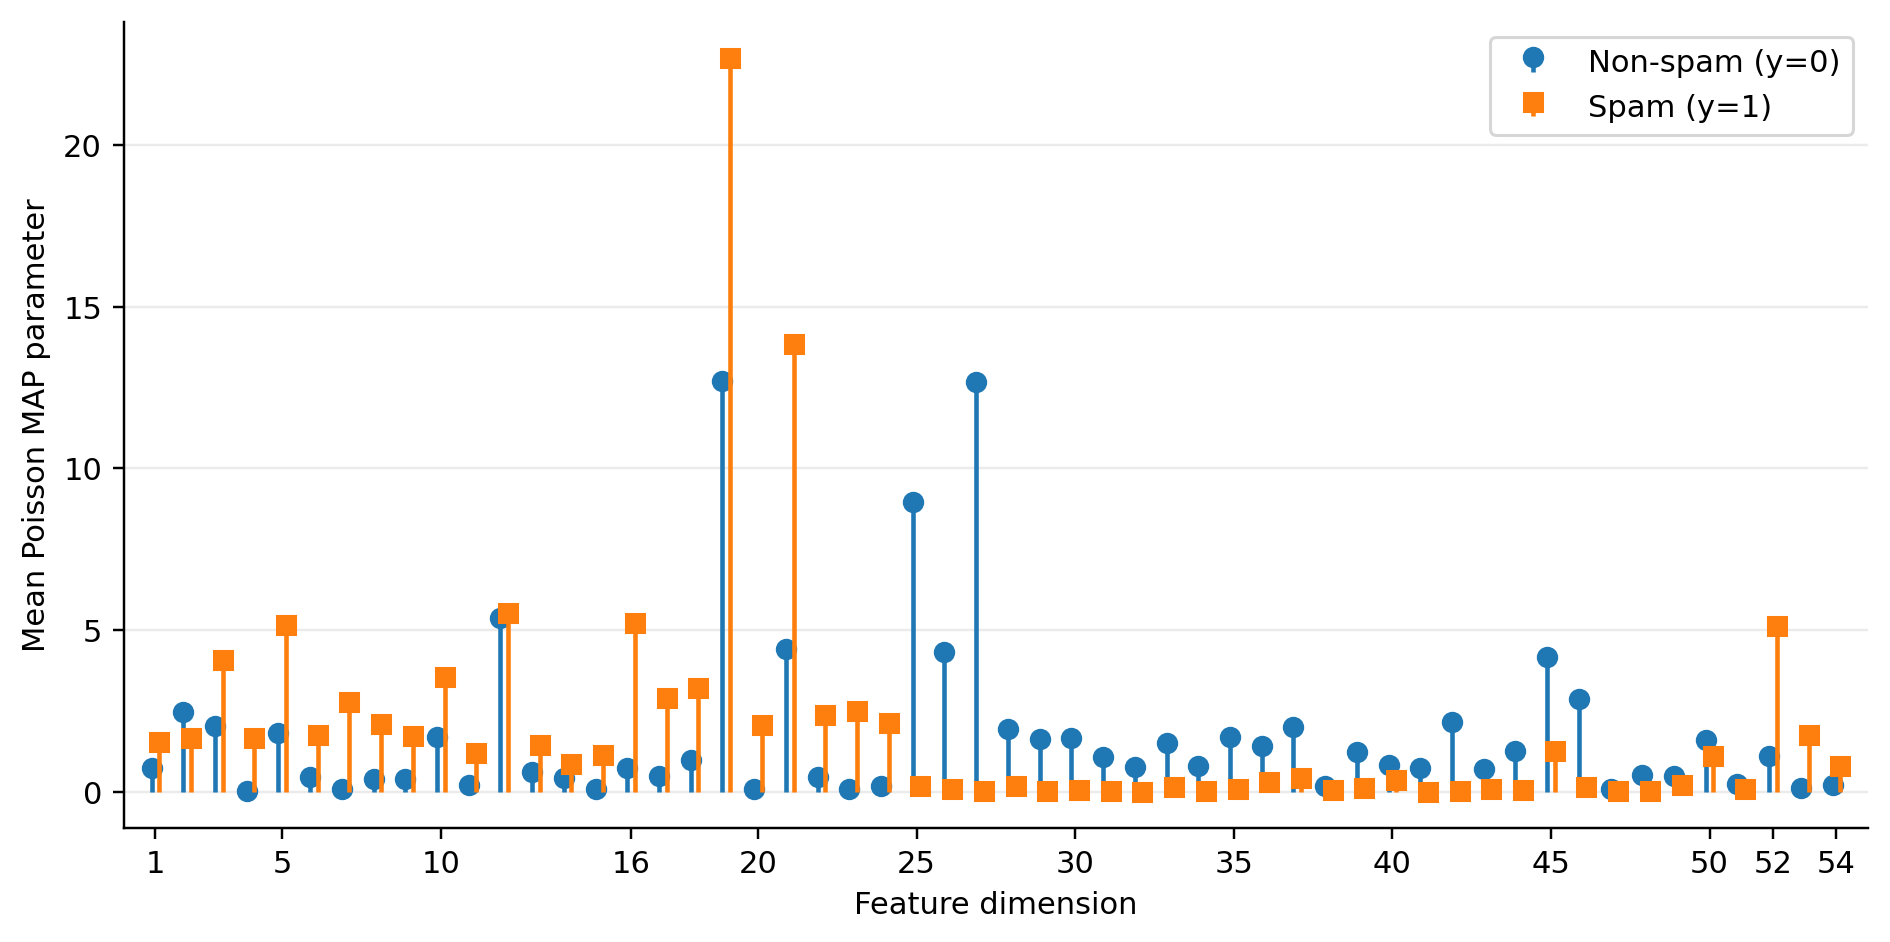
\includegraphics[width=0.93\linewidth]{p2b_poisson_parameters.png}
\captionof{figure}{Mean Poisson MAP parameters for both classes. Stems are shifted slightly to distinguish the classes.}
\end{center}
Dimension 16 is the word ``free'' and dimension 52 is ``!''.
Their mean rates for non-spam and spam are, respectively,
\begin{center}
\begin{tabular}{lrr}\toprule
Feature & Non-spam & Spam\\\midrule
16: free & 0.73960 & 5.21371\\
52: ! & 1.09615 & 5.12924\\\bottomrule
\end{tabular}
\end{center}
Both rates are larger for spam, so higher values of either feature favor spam through a positive contribution to the log score difference.

\clearpage
\subsection*{(c) Logistic regression by steepest ascent}
Map each label 0 to $-1$ and retain $+1$. Append a constant $+1$ to each row, giving $a_i\in\mathbb R^{55}$.
For a training fold, the sum log likelihood and its gradient are
\begin{align*}
\mathcal L(w)&=\sum_{i\in\mathcal T}\log\sigmoid(y_i a_i^Tw)
=-\sum_{i\in\mathcal T}\log(1+e^{-y_i a_i^Tw}),\\
\nabla\mathcal L(w)&=\sum_{i\in\mathcal T}y_i a_i\sigmoid(-y_i a_i^Tw),
\qquad\sigmoid(z)=\frac1{1+e^{-z}}.
\end{align*}
Starting at $w^{(0)}=0$, perform exactly 1,000 updates
\[w^{(t)}=w^{(t-1)}+\eta\nabla\mathcal L(w^{(t-1)}),
\qquad\eta=\frac{0.01}{4600}\approx2.173913\times10^{-6}.\]
The denominator is 4,600 as specified, even though a training fold has 4,140 rows. No penalty is added.
\begin{center}
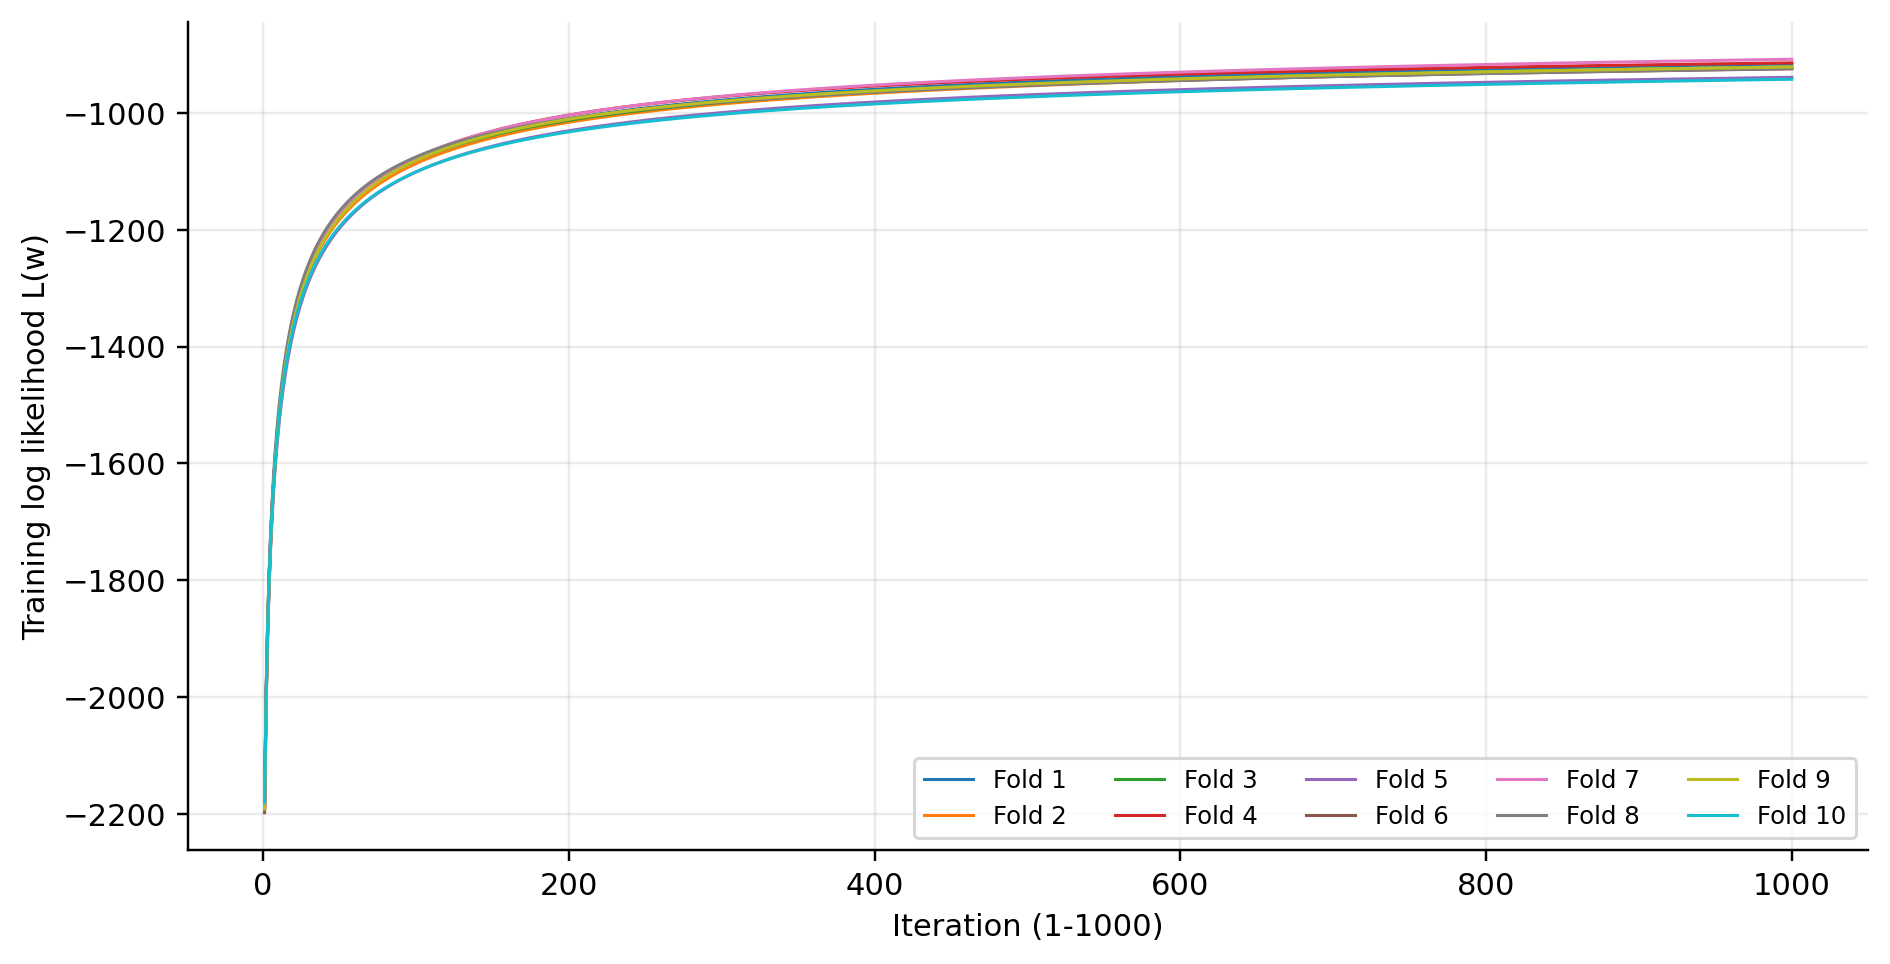
\includegraphics[width=0.96\linewidth]{p2c_steepest_ascent.png}
\captionof{figure}{Training log likelihood after each steepest-ascent update, for all ten training runs in one figure.}
\end{center}
Every run starts at $-4140\log2=-2869.62933$. The curves increase toward higher likelihood.
After 1,000 steps, the objectives range from $-942.37473$ to $-908.17458$.
The fixed small step produces gradual improvement.

\clearpage
\subsection*{(d) Newton's method: derivation and implementation}
Write $g_t=\nabla\mathcal L(w_t)$ and $H_t=\nabla^2\mathcal L(w_t)$. For the quadratic approximation
\[Q_t(w)=\mathcal L(w_t)+(w-w_t)^Tg_t+\tfrac12(w-w_t)^TH_t(w-w_t),\]
the stationarity equation is
\[\nabla Q_t(w)=g_t+H_t(w-w_t)=0
\quad\Longrightarrow\quad w_{t+1}=w_t-H_t^{-1}g_t.\]
For logistic regression, let $q_i=\sigmoid(y_i a_i^Tw_t)$ and $R_t=\operatorname{diag}(q_i(1-q_i))$.
Differentiating the gradient gives
\[H_t=-\sum_{i\in\mathcal T}a_i a_i^Tq_i(1-q_i)=-A^TR_tA.\]
The Hessian is negative semidefinite, so a well-defined stationary point maximizes the approximation. Substitution gives
\[w_{t+1}=w_t+(A^TR_tA)^{-1}A^T[y\odot\sigmoid(-y\odot Aw_t)].\]
The implementation solves $(A^TR_tA)\Delta_t=g_t$ and sets $w_{t+1}=w_t+\Delta_t$, using a least-squares pseudoinverse solve rather than an explicit inverse.
Starting at zero, it performs all 100 unregularized full Newton updates for every fold.
\begin{center}
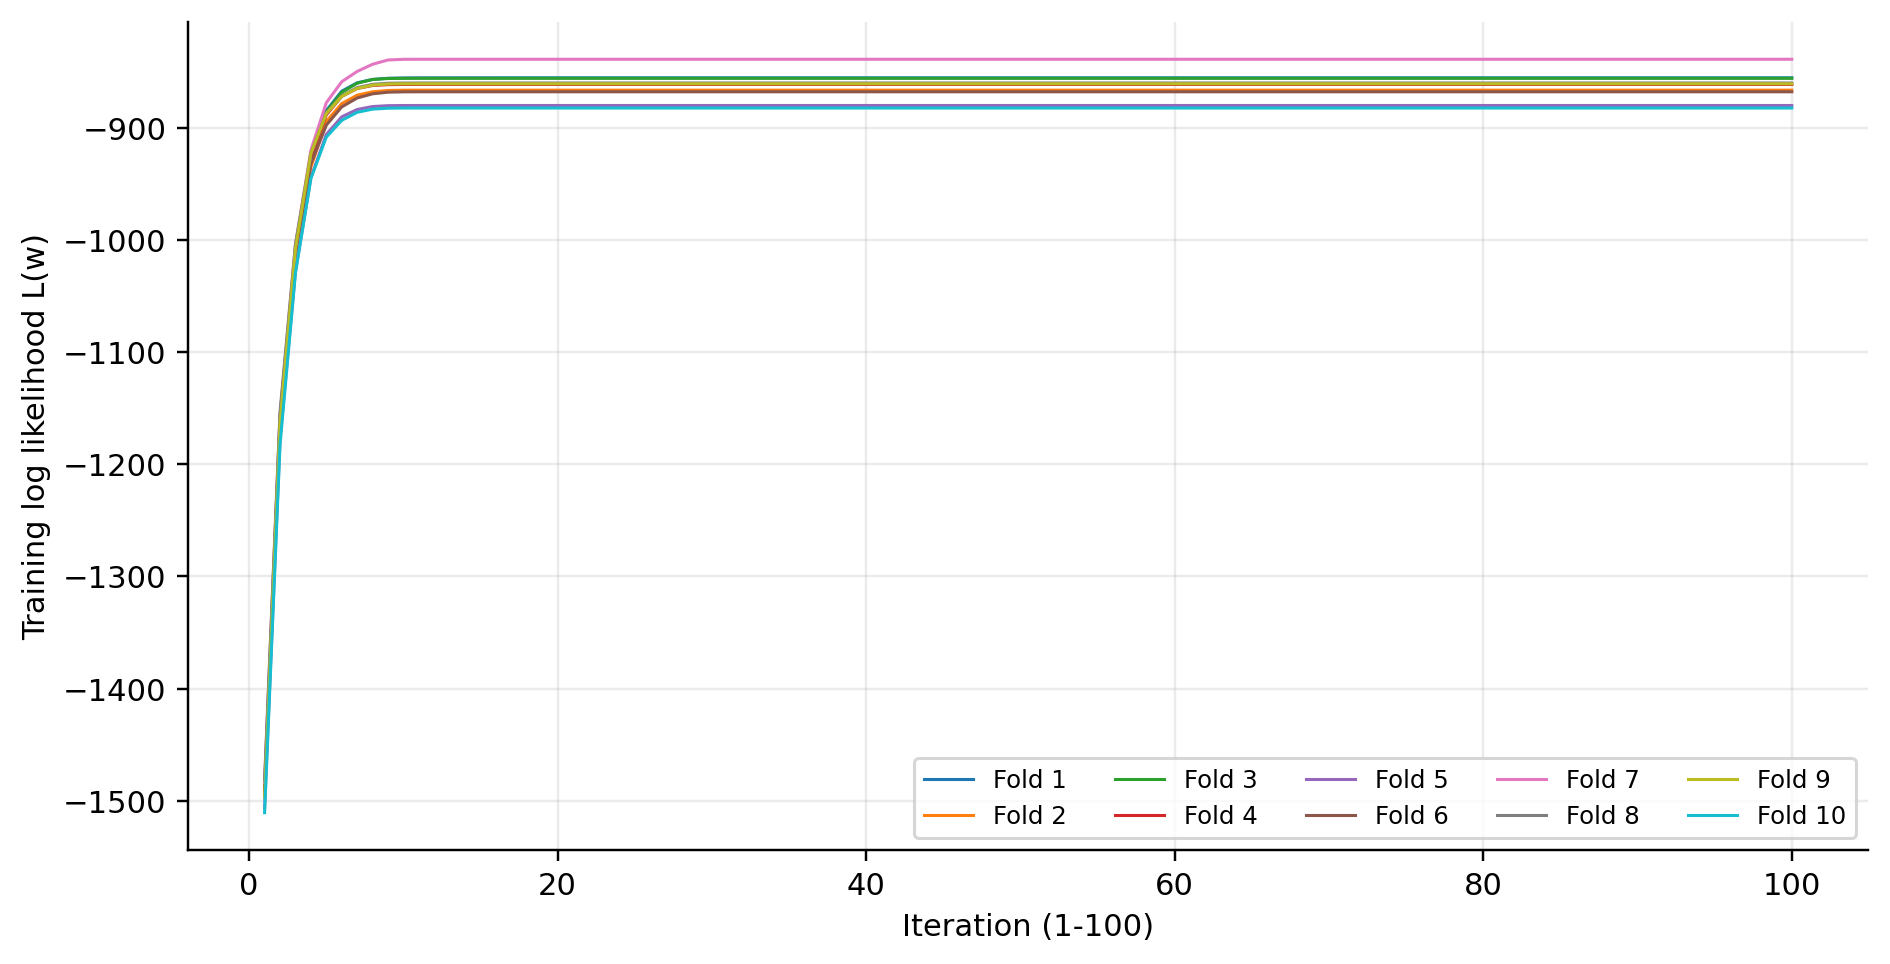
\includegraphics[width=0.85\linewidth]{p2d_newton.png}
\captionof{figure}{Training log likelihood after each Newton update, for all ten training runs in one figure.}
\end{center}
\subsection*{(e) Newton logistic regression test results}
Predict spam if $a^Tw\ge0$, equivalently $\sigmoid(a^Tw)\ge1/2$.
\begin{center}
\begin{tabular}{lrr}\toprule
Ground truth & Predicted 0 & Predicted 1\\\midrule
0 (non-spam) & 2647 & 140\\
1 (spam) & 220 & 1593\\\bottomrule
\end{tabular}\qquad
\begin{minipage}{0.35\linewidth}
\[\text{Accuracy}=\frac{2647+1593}{4600}=92.1739\%.\]
\end{minipage}
\end{center}
The entries sum to 4,600. Newton's method reaches higher training likelihood than the 1,000 steepest-ascent steps and makes 230 fewer held-out mistakes than naive Bayes on these folds.

\clearpage
\section*{Problem 3: AdaBoost with bootstrap least squares}
The toy data contain $n=1000$ rows with labels $\pm1$. The third feature is already one, so no intercept is appended.
Initialize $D_1(i)=1/n$ and $F_0(x)=0$. For $t=1,\ldots,2500$:
\begin{enumerate}
\item Sample a bootstrap multiset $B_t$ of exactly $n$ indices with replacement from $D_t$ and fit
\[\beta_t=\arg\min_\beta\sum_{j\in B_t}(y_j-x_j^T\beta)^2.\]
Repeated sampled indices are retained as repeated rows.
\item Set $h_t(x)=\operatorname{sign}(x^T\beta_t)$, assigning zero to $+1$, and evaluate on the original training set:
\[\epsilon_t=\sum_iD_t(i)\ind\{h_t(x_i)\ne y_i\}.\]
If $\epsilon_t>1/2$, negate the whole $\beta_t$, including its offset, and recompute the error.
\item Update the ensemble and sampling distribution:
\begin{align*}
\alpha_t&=\frac12\log\frac{1-\epsilon_t}{\epsilon_t},
&F_t(x)&=F_{t-1}(x)+\alpha_t h_t(x),\\
D_{t+1}(i)&=\frac{D_t(i)e^{-\alpha_t y_i h_t(x_i)}}{Z_t},
&Z_t&=\sum_iD_t(i)e^{-\alpha_t y_i h_t(x_i)}.
\end{align*}
\end{enumerate}
The boosted prediction is $\operatorname{sign}F_t(x)$, with zero assigned to $+1$.
Sampling uses seed 4721. If $\epsilon_t=1/2$, then $\alpha_t=0$ and the ensemble is unchanged; all 2,500 rounds are retained.
\subsection*{(a) Empirical error and upper bounds}
The mistake indicator satisfies $\ind\{f_{\rm boost}^{(t)}(x_i)\ne y_i\}\le e^{-y_iF_t(x_i)}$. Hence
\begin{align*}
\widehat R_t&=\frac1n\sum_i\ind\{f_{\rm boost}^{(t)}(x_i)\ne y_i\}\\
&\le\frac1n\sum_i e^{-y_iF_t(x_i)}
=\prod_{s=1}^tZ_s
=\prod_{s=1}^t2\sqrt{\epsilon_s(1-\epsilon_s)}.
\end{align*}
Unrolling the normalized distribution updates from $D_1(i)=1/n$ yields the product identity. The selected coefficient gives
\[Z_s=(1-\epsilon_s)e^{-\alpha_s}+\epsilon_s e^{\alpha_s}
=2\sqrt{\epsilon_s(1-\epsilon_s)}.\]
Writing $\gamma_s=1/2-\epsilon_s$ and applying $\log(1-u)\le-u$ gives the common looser bound
\[\widehat R_t\le\prod_{s=1}^t\sqrt{1-4\gamma_s^2}
\le\exp\!\left(-2\sum_{s=1}^t\gamma_s^2\right).\]
Both upper bounds are plotted with the empirical error.

\clearpage
\subsection*{(a) Training error and upper bounds}
\begin{center}
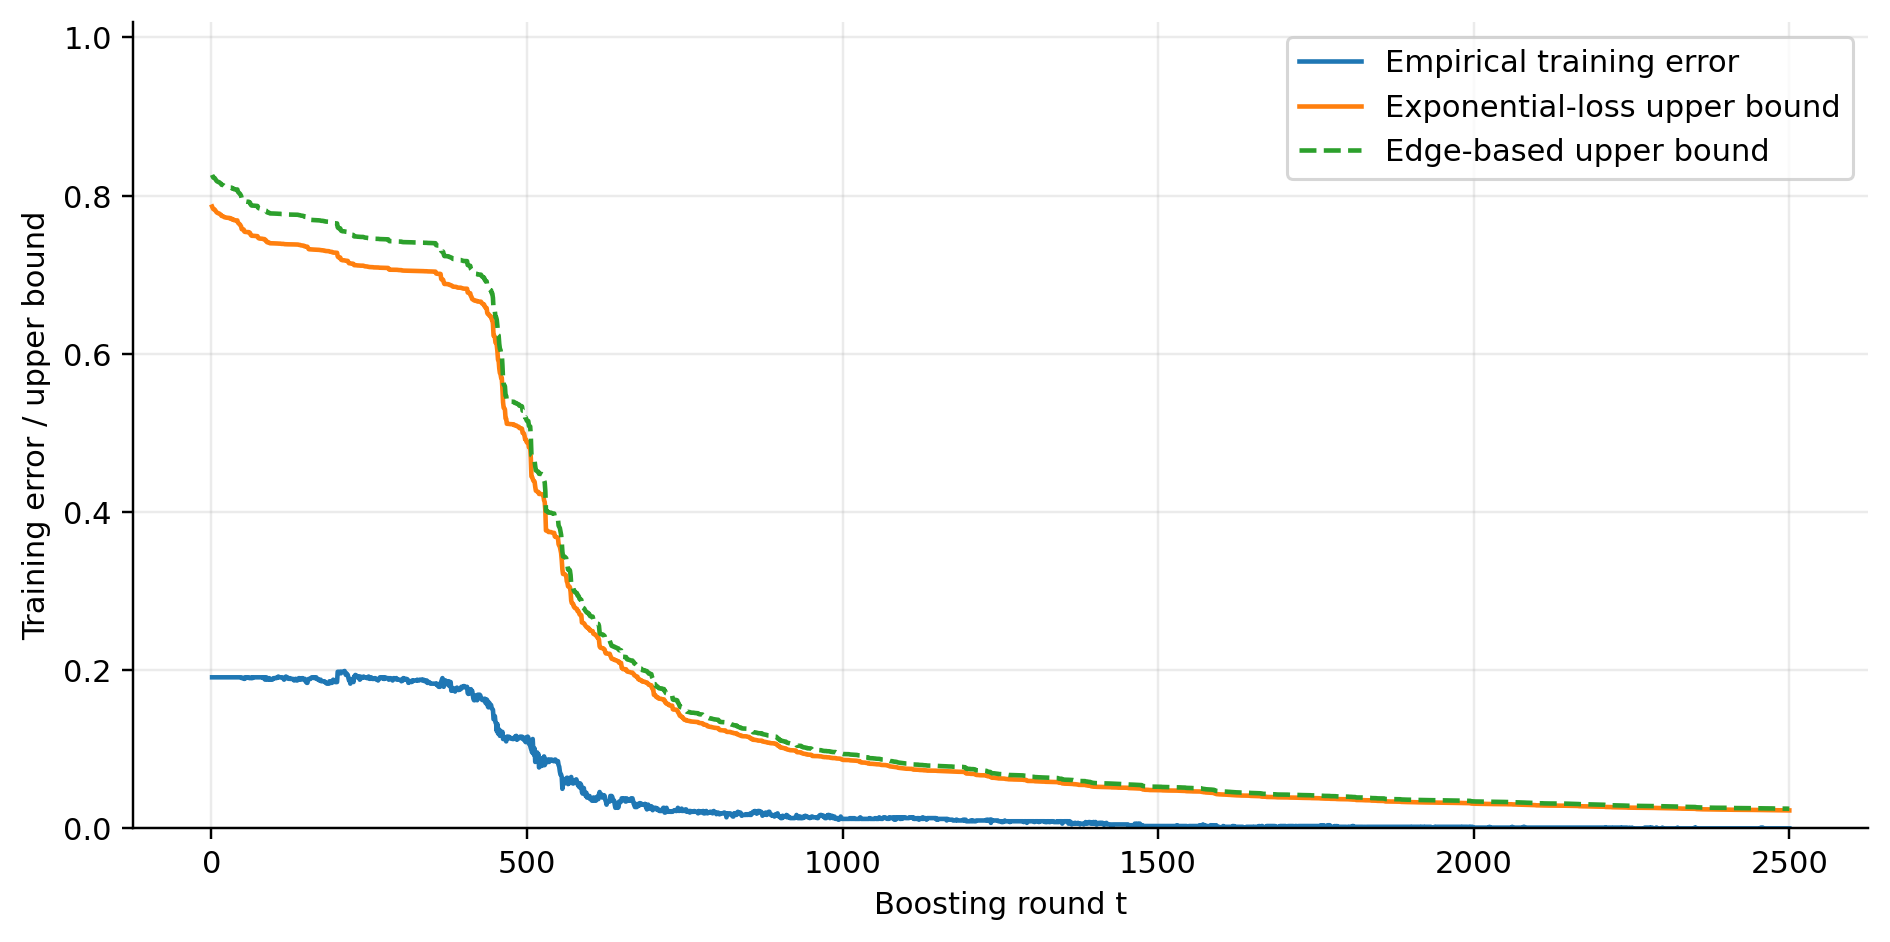
\includegraphics[width=0.87\linewidth]{p3a_training_error_bound.png}
\captionof{figure}{Training error, exact exponential-loss bound, and looser edge-based bound over all 2,500 rounds.}
\end{center}
The final classifier makes $0/1000$ training mistakes. At round 2,500 the exponential-loss bound is $0.0227164$ and the edge-based bound is $0.0248033$.
The bounds hold at every round; the empirical error itself need not decrease at every round. These are training results, not estimates of test error.
\subsection*{(b) Average distribution on the data}
Average the probabilities used for bootstrap sampling:
\[\overline D(i)=\frac1{2500}\sum_{t=1}^{2500}D_t(i).\]
\begin{center}
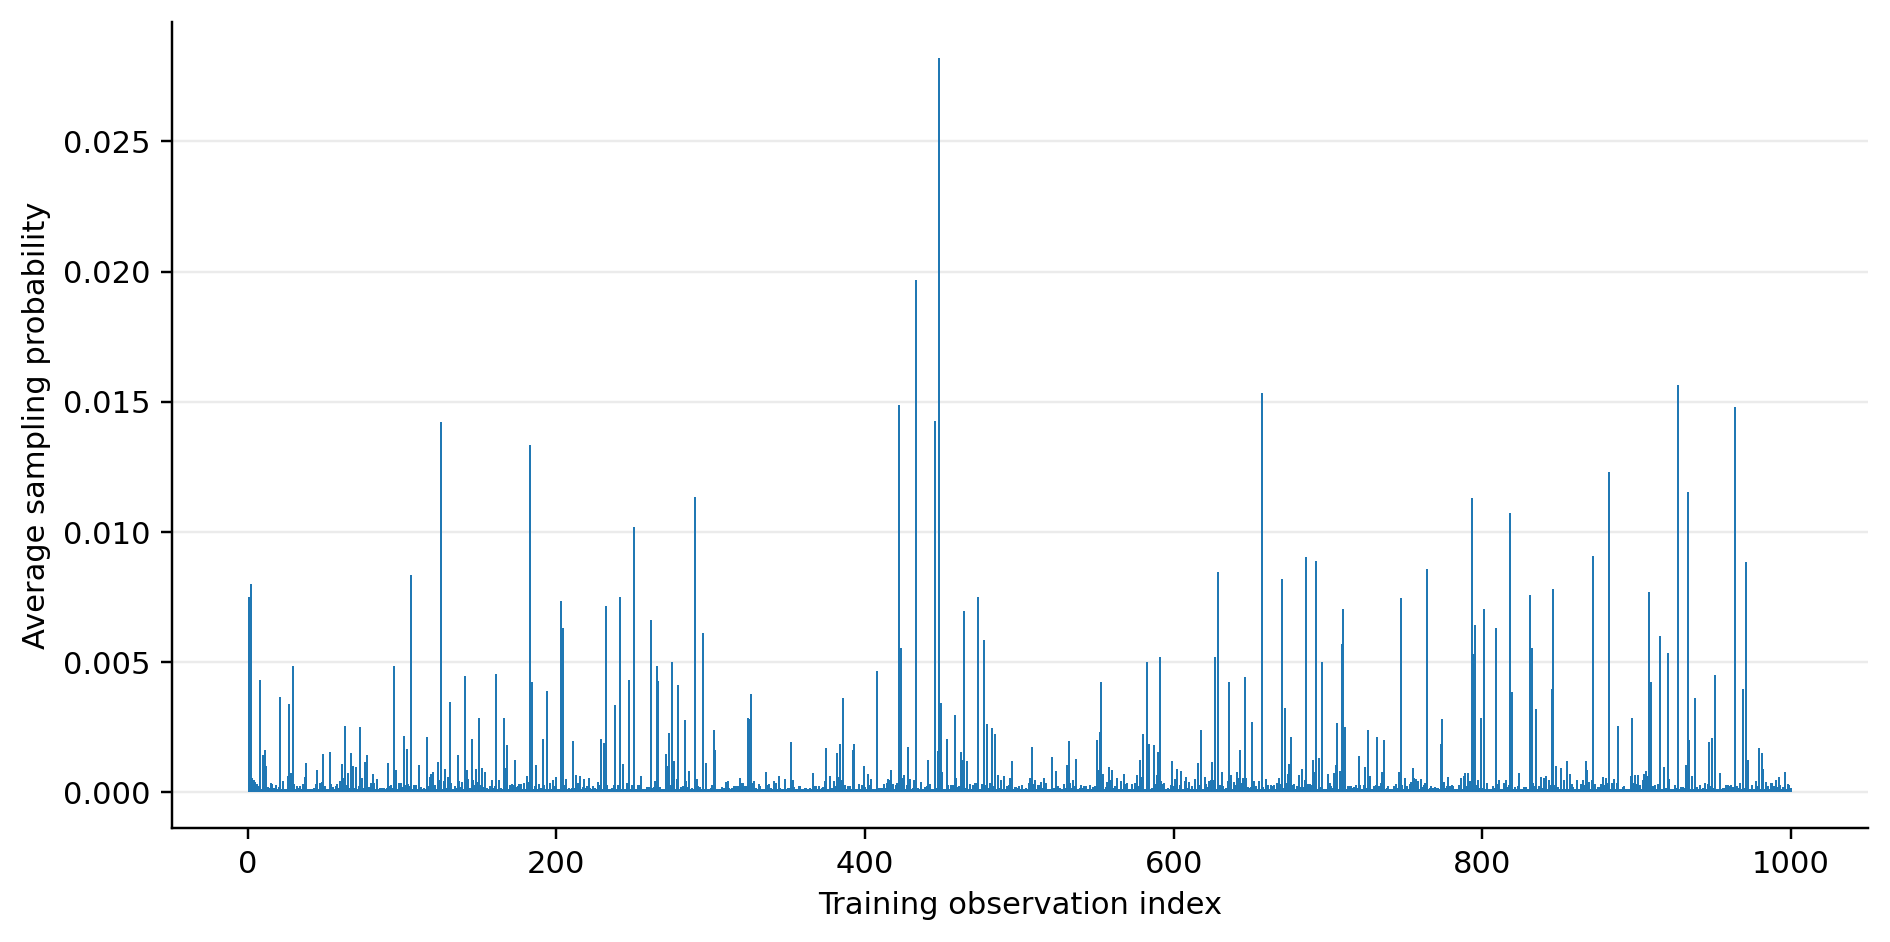
\includegraphics[width=0.87\linewidth]{p3b_average_distribution.png}
\captionof{figure}{Stem plot of the average sampling distribution over all 1,000 observations.}
\end{center}
The probabilities sum to one and concentrate on repeatedly difficult observations.
Observation 448 has the largest mean probability, approximately $0.02820$, compared with $0.001$ initially.

\clearpage
\subsection*{(c) Weak-classifier errors and ensemble coefficients}
\begin{center}
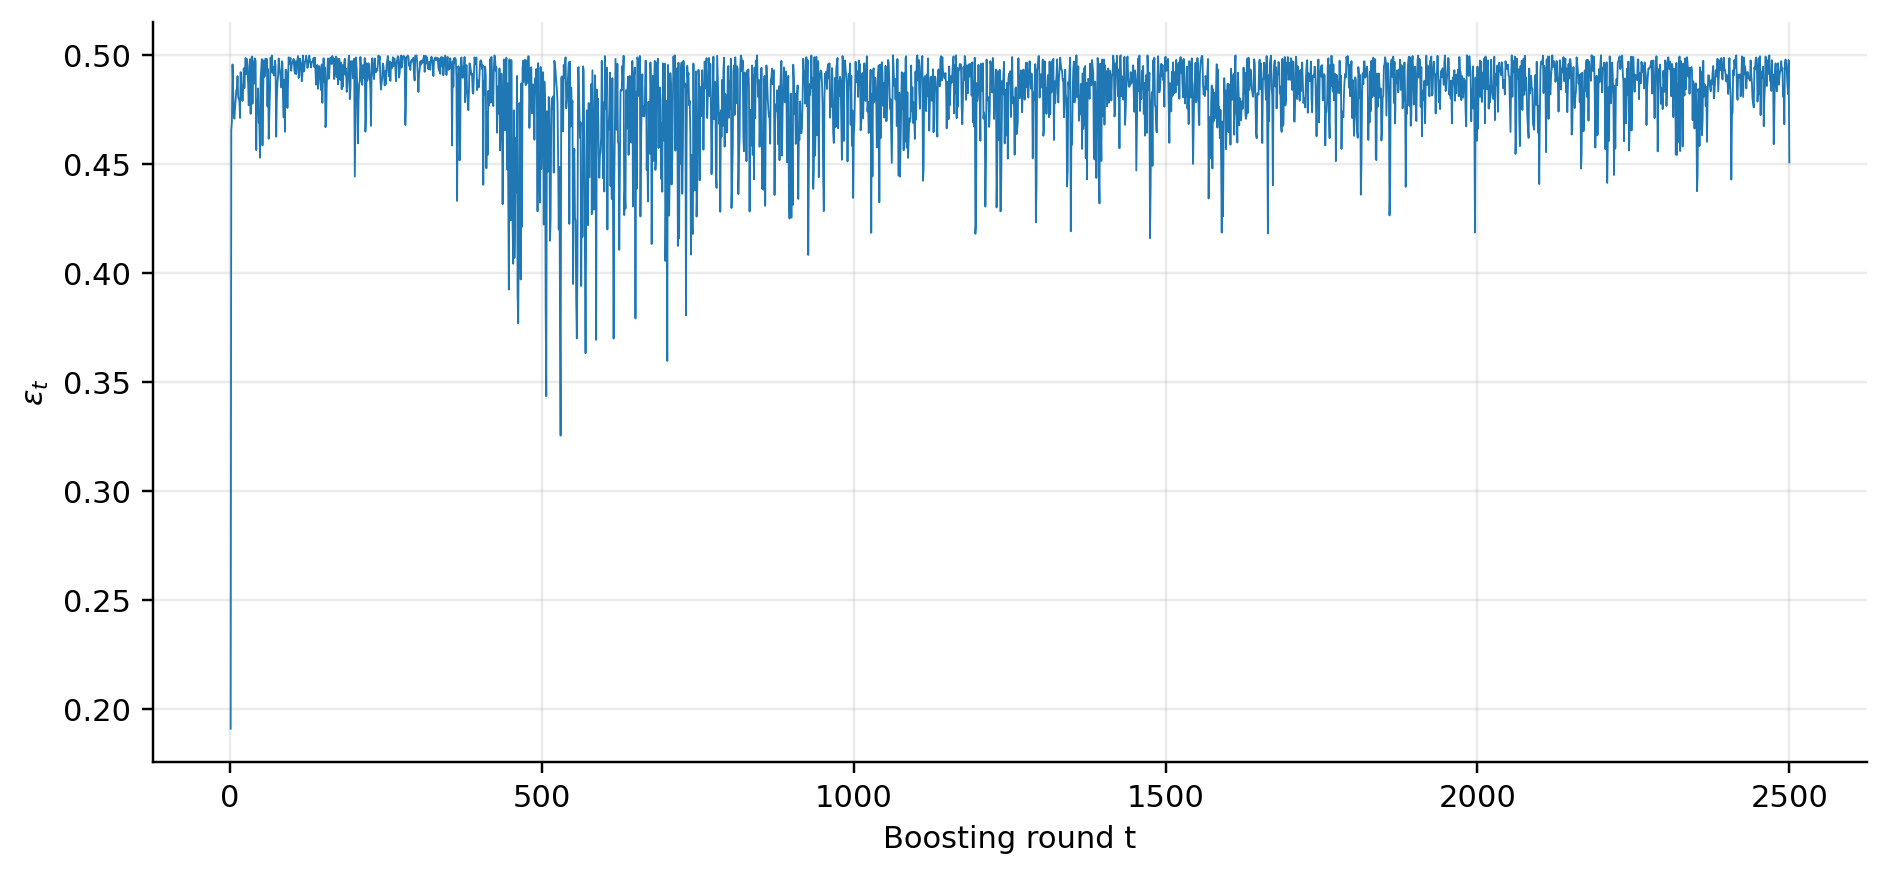
\includegraphics[width=0.97\linewidth]{p3c_epsilon.png}
\captionof{figure}{Weighted weak-classifier error $\epsilon_t$, after sign reversals, over 2,500 rounds.}
\end{center}
\begin{center}
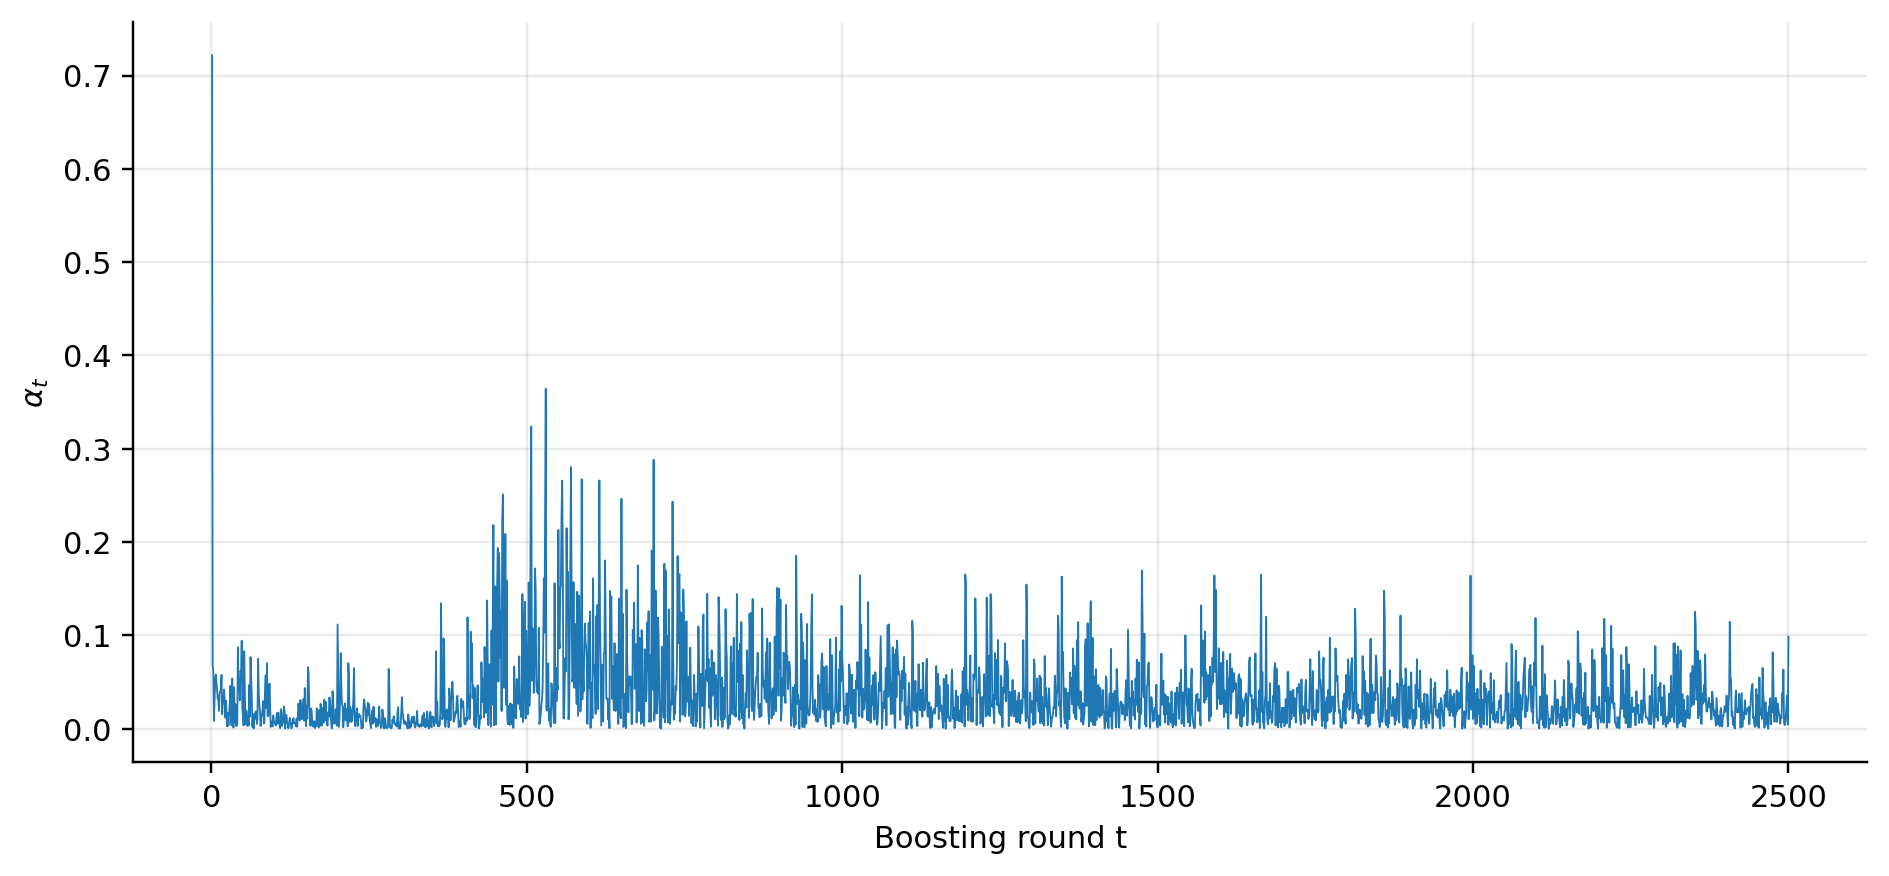
\includegraphics[width=0.97\linewidth]{p3c_alpha.png}
\captionof{figure}{AdaBoost coefficient $\alpha_t=\tfrac12\log[(1-\epsilon_t)/\epsilon_t]$, shown in a separate figure.}
\end{center}
The errors range from $0.191$ to $0.5$; coefficients range from 0 to $0.72176$.
Smaller weighted errors receive larger coefficients, while errors close to chance receive small coefficients.
Exactly $\epsilon_t=1/2$ gives $\alpha_t=0$. Sign reversal was applied in 935 rounds before recording errors and coefficients.
The variation reflects the changing distribution and the random bootstrap samples.
\end{document}
